% !TEX root = ../main.tex
% Appendix A
\chapter{Supplementary Material}
\label{AppendixA}

% REWIRED 2026-08-14. This appendix now carries everything displaced from the body by the
% Mean Teacher rewire: the from-scratch MONAI study and the retired ablations. The
% appendix is NOT word-counted, so it is the right home for that material -- but it is still
% read, so it must stay accurate and must not contradict the body.
%
% ROUGH DRAFT: split into further appendices if navigation suffers.

\section{Dataset manifests}

\begin{itemize}
  \item Exact ATM'22 identifiers in the labelled, label-withheld, external validation and
  sealed test partitions, plus the split-generation seed and code version.
  \item Record that the split is a frozen manifest rather than a re-runnable splitter, and
  show the consequence: re-running the original count-based splitter over the enlarged
  inventory would have moved most previously held-out cases into training. Give the numbers.
  \item Declare which identifiers were added to the unlabelled pool only, and confirm no
  validation or test case entered any training pool.
  \item nnU-Net internal fold membership listed separately from the external project split,
  including the exact four-case internal validation set per fold.
  \item AeroPath case identifiers, with confirmation of external-evaluation-only use.
\end{itemize}

\section{Loss and objective definitions}

\begin{itemize}
  \item Full equations: weighted cross-entropy, soft Dice, differentiable skeletonisation,
  topology sensitivity, topology precision, soft clDice, and the consistency term as
  $1-F_1$ of the two directional terms at smoothing constant one.
  \item Document numerical stabilisers, erosion depth, pooling kernels, reduction over batch
  and channel dimensions, and the exact accumulation of ridge residuals.
  \item Derive and state the property referenced in the Discussion: for fractional maps the
  unthresholded objective is not zero at equality, hence a residual sharpening component.
  Show the algebra --- this is a load-bearing claim, so it should end in a result rather than
  a gesture.
\end{itemize}

Algorithm~\ref{alg:soft-skeleton} gives the skeletonisation of
Equations~\eqref{eq:morph}--\eqref{eq:accumulate} in the form it is implemented, with the
pooling kernels and the accumulation order made explicit.

\begin{algorithm}[htbp]
  \caption[Differentiable soft skeletonisation]{Differentiable soft skeletonisation, after Shit
  et al.~\cite{shit2021cldice}. \textsc{MinPool} and \textsc{MaxPool} are unit-stride pooling
  with shape-preserving padding; the three directional minimum pools compose to the
  six-neighbour erosion of Equation~\eqref{eq:morph}, and the cubic maximum pool is the
  26-neighbour dilation. Every operation is differentiable, so gradient reaches $X$ through each
  retained residual. Called on the student probability map and on the thresholded teacher tree
  with $K=10$.}
  \label{alg:soft-skeleton}
  \begin{algorithmic}[1]
    \Require probability map $X\in[0,1]^{D\times H\times W}$, erosion depth $K$
    \Ensure soft skeleton $S\in[0,1]^{D\times H\times W}$
    \Function{Erode}{$X$}\Comment{$\mathcal{E}$}
      \State \Return $\min\!\big(\textsc{MinPool}_{3\times1\times1}(X),\,
                                 \textsc{MinPool}_{1\times3\times1}(X),\,
                                 \textsc{MinPool}_{1\times1\times3}(X)\big)$
    \EndFunction
    \Function{Open}{$X$}\Comment{$\mathcal{O}=\mathcal{D}\circ\mathcal{E}$}
      \State \Return $\textsc{MaxPool}_{3\times3\times3}(\Call{Erode}{X})$
    \EndFunction
    \Statex
    \State $S \gets \operatorname{ReLU}\!\left(X-\Call{Open}{X}\right)$
      \Comment{$\delta^{(0)}$, Equation~\eqref{eq:residual}}
    \For{$k \gets 1$ \textbf{to} $K$}
      \State $X \gets \Call{Erode}{X}$ \Comment{$X^{(k)}$}
      \State $\delta \gets \operatorname{ReLU}\!\left(X-\Call{Open}{X}\right)$
        \Comment{$\delta^{(k)}$}
      \State $S \gets S+\operatorname{ReLU}\!\left(\delta-S\,\delta\right)$
        \Comment{probabilistic union, Equation~\eqref{eq:accumulate}}
    \EndFor
    \State \Return $S$
  \end{algorithmic}
\end{algorithm}

Figure~\ref{fig:soft-skeleton-operator} states the operator geometry that the main-text
figure demonstrates but cannot show: the two structuring neighbourhoods are different shapes,
so the composition is the implemented soft opening and not an adjoint morphological pair.
Figure~\ref{fig:soft-skeleton-extended} then expands the main-text illustration to show
intermediate erosion depths on a second patch. All panels are computed from three-dimensional
probability crops; only their presentation is two-dimensional.

\begin{figure}[htbp]
  \centering
  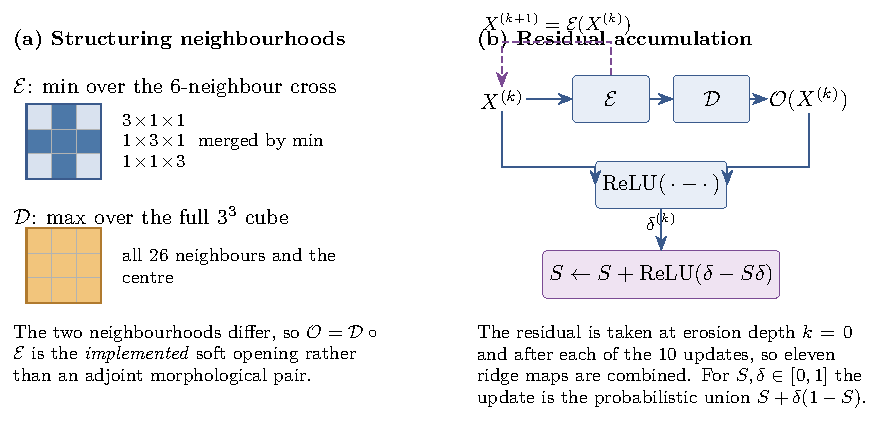
\includegraphics[width=\linewidth]{Figures/pdf/methods/cldice/soft_skeleton_operator.pdf}
  \caption[Soft-skeletonisation operators]{The implemented soft skeleton.
  (a)~Erosion takes the minimum over the six face-connected neighbours and the centre, built
  from three directional minimum pools; dilation takes the maximum over the full $3^3$ cube.
  (b)~Each erosion depth contributes the positive residual left by the opening, and the
  residuals are combined by a probabilistic union so that evidence is not double-counted.
  Operator geometry and dataflow only; no patient data is shown.}
  \label{fig:soft-skeleton-operator}
\end{figure}

\begin{figure}[htbp]
  \centering
  \begin{subfigure}[t]{0.32\textwidth}
    \centering
    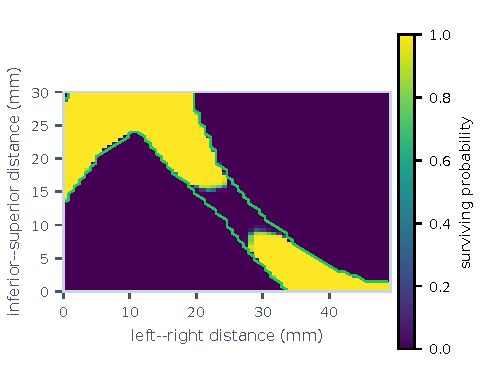
\includegraphics[width=\linewidth]{Figures/pdf/methods/cldice/soft_erosion_depth_0.pdf}
    \caption{Depth 0.}
  \end{subfigure}\hfill
  \begin{subfigure}[t]{0.32\textwidth}
    \centering
    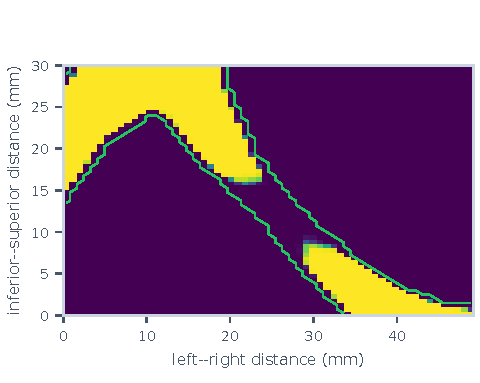
\includegraphics[width=\linewidth]{Figures/pdf/methods/cldice/soft_erosion_depth_1.pdf}
    \caption{Depth 1.}
  \end{subfigure}\hfill
  \begin{subfigure}[t]{0.32\textwidth}
    \centering
    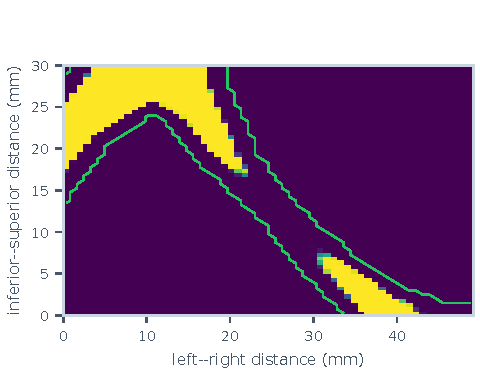
\includegraphics[width=\linewidth]{Figures/pdf/methods/cldice/soft_erosion_depth_3.pdf}
    \caption{Depth 3.}
  \end{subfigure}

  \medskip
  \begin{subfigure}[t]{0.32\textwidth}
    \centering
    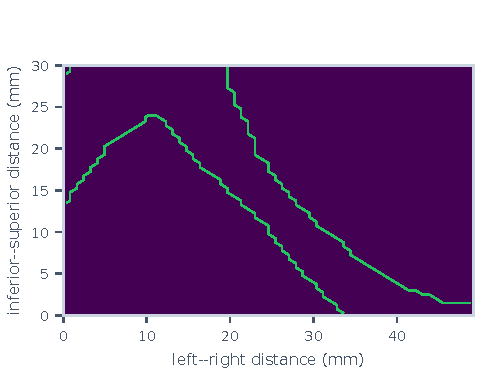
\includegraphics[width=\linewidth]{Figures/pdf/methods/cldice/soft_erosion_depth_7.pdf}
    \caption{Depth 7.}
  \end{subfigure}\hfill
  \begin{subfigure}[t]{0.32\textwidth}
    \centering
    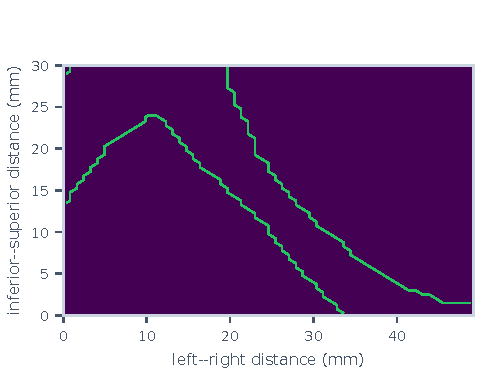
\includegraphics[width=\linewidth]{Figures/pdf/methods/cldice/soft_erosion_depth_10.pdf}
    \caption{Depth 10.}
  \end{subfigure}\hfill
  \begin{subfigure}[t]{0.32\textwidth}
    \centering
    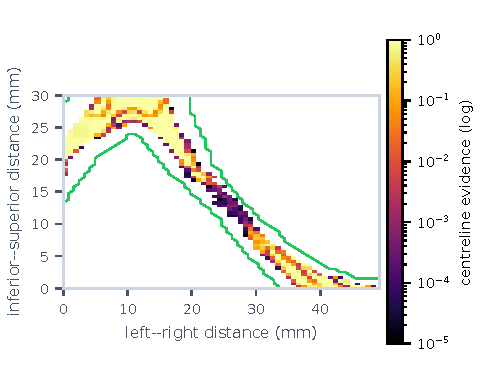
\includegraphics[width=\linewidth]{Figures/pdf/methods/cldice/soft_skeleton_accumulated.pdf}
    \caption{Accumulated $S(p_T)$.}
  \end{subfigure}
  \caption[Extended soft-erosion sequence]{Extended soft-erosion sequence for the real
  airway patch, taken from the final fold-0 EMA teacher. Repeated directional
  minimum pooling removes successive tube layers; ridge residuals extracted at depths
  0--10 are combined into the final graded soft skeleton.}
  \label{fig:soft-skeleton-extended}
\end{figure}

\section{Metric definitions and edge cases}

\begin{itemize}
  \item Pseudocode for native and connected scoring, tree-length detection, branch parsing,
  topology precision and the corrected hard clDice.
  \item Truth table for empty prediction, empty target, both empty, and non-empty disjoint
  trees; document the corrected behaviour and the exact magnitude by which it changed a
  previously reported baseline mean.
  \item Define 6- and 26-neighbour connectivity, the trachea-seed window construction from
  the affine, and the largest-component fallback rule.
  \item Record the ground-truth support inconsistency across historical scoring paths, which
  cases it affects, and the rescoring policy applied before the final tables.
  \item State explicitly why the legacy wall-shell distance bin is excluded from anatomical
  claims, so a reader encountering it in the repository is not misled.
  \item Official-evaluator parity results when complete.
\end{itemize}

\section{Training and inference configurations}

\begin{itemize}
  \item Table of all reportable runs: semantic run name, data, pool, fold, architecture,
  patch, sampling, objective, warm-up and ramp, optimiser, schedule, epochs, checkpoint
  selector and inference settings.
  \item nnU-Net plan summary: target spacing, median image size, patch size, batch size,
  normalisation, deep supervision and mirroring status, ensemble membership.
  \item Full online augmentation specification with per-transform probabilities and ranges,
  plus the additional student perturbation amplitudes and their start epoch.
  \item Exposure arithmetic worked through for each arm: steps per epoch, epochs, total
  labelled and unlabelled patch presentations, per-case draws, and distinct cases sampled per
  epoch.
  \item Hardware and software table: GPU, CUDA, PyTorch, MONAI, nnU-Net versions, operating
  system, git commit, approximate training and inference wall-clock time, and resume history
  for any run that exceeded its walltime.
\end{itemize}

\section{Extended results for the main study}

\begin{itemize}
  \item Per-case tables for every matched pair, with paired differences and bootstrap
  intervals.
  \item Native versus connected audits at 6- and 26-neighbour connectivity, including the
  fragmentation-sensitive cases and the retained-foreground fractions.
  \item Full parsed diagnostic series behind the mid-training measurements: gradient
  contribution and cosine per epoch, teacher evidence statistics, counterfactual losses and
  the objective decomposition. The body reports summary statistics; the appendix carries the
  series and states the sampling frequency.
  \item Checkpoint comparison across all arms under one policy, with the alternative policy as
  a full sensitivity table.
  \item Offline pseudo-labelling per-case differences.
  \item AeroPath per-case table and representative failures once the external test is run.
  \item Deduplicated score inventory for the nnU-Net arms this dissertation reports
  (Table~\ref{tab:nnunet-all-scores}), so that any number quoted in the body can be traced back
  to a single score file.
\end{itemize}

Table~\ref{tab:nnunet-all-scores} collects every arm the body relies on, together with the
reference rungs it is measured against. It reports cohort means only; per-case
values are in the tables above. One score file was selected per prediction directory --- the most
recent complete \texttt{hard-cldice-v2} evaluation at six-neighbour connectivity, falling back to
the original single-connectivity report where no rescored file exists --- and prediction
directories whose means agree to full double precision were collapsed to a single row. The
supervised @110 predictions are the only such collision: two directories hold the same masks under
different names, and appear once here.

\begin{table}[htbp]
  \centering
  \footnotesize
  \setlength{\tabcolsep}{3pt}
  \caption[Deduplicated nnU-Net scores on the frozen external cohorts]{Cohort-mean scores for
  each reported nnU-Net arm, on the native (RAW) mask and after trachea-seeded
  six-neighbour largest-connected-component selection (LCC-6). Dice and precision are voxel-wise;
  TLD is tree length detected and BD is branch detected. All ATM'22 rows use the frozen external
  VAL-20 cohort \{016, 027, 028, 033, 034, 043, 044, 046, 056, 068, 078, 081, 087, 116, 125, 126,
  147, 150, 151, 152\}; the final row is the AeroPath out-of-distribution cohort and shares no
  cases with it. RAW is the primary output and LCC-6 is a sensitivity, not a competing headline.}
  \label{tab:nnunet-all-scores}
  \begin{tabular}{llcrrrrrrrr}
    \toprule
    & & & \multicolumn{4}{c}{RAW (native)} & \multicolumn{4}{c}{$+$ trachea-LCC-6} \\
    \cmidrule(lr){4-7} \cmidrule(lr){8-11}
    Run & Dir. & $n$ & Dice & TLD & BD & Prec. & Dice & TLD & BD & Prec. \\
    \midrule
    \multicolumn{11}{l}{\itshape Supervised nnU-Net, 110 labelled cases (full volume)} \\
    \quad No deep supervision/no mirroring, fold~0 & \texttt{111\_nods\_f0} & 20 & 0.925 & 0.933 & 0.882 & 0.949 & 0.925 & 0.917 & 0.859 & 0.953 \\
    \quad Stock 5-fold ensemble $+$ TTA & \texttt{111\_5f} & 20 & 0.926 & 0.938 & 0.890 & 0.944 & 0.926 & 0.926 & 0.870 & 0.947 \\
    \addlinespace
    \multicolumn{11}{l}{\itshape Supervised and offline-SSL controls, 20 labelled cases (full volume)} \\
    \quad Dice fold~0* & \texttt{120\_dice} & 20 & 0.924 & 0.914 & n/a & 0.934 & 0.919 & 0.875 & 0.798 & 0.942 \\
    \quad clDice fold~0* & \texttt{120\_cldice} & 20 & 0.923 & 0.920 & n/a & 0.927 & 0.916 & 0.883 & 0.810 & 0.933 \\
    \quad Offline pseudo-label SSL & \texttt{121} & 20 & 0.921 & 0.899 & n/a & 0.943 & 0.921 & 0.879 & 0.782 & 0.945 \\
    \addlinespace
    \multicolumn{11}{l}{\itshape Historical ignore-label Mean Teacher, 20 labelled + 90 unlabelled (full volume)} \\
    \quad Cold start & \texttt{122} & 20 & 0.810 & 0.423 & n/a & 0.859 & 0.818 & 0.387 & 0.315 & 0.890 \\
    \quad Warm start, symmetric\textsuperscript{\ddag} & \texttt{122\_sym} & 20 & 0.923 & 0.948 & n/a & 0.922 & 0.926 & 0.922 & 0.876 & 0.937 \\
    \quad Warm symmetric, lung-ROI inference\textsuperscript{\ddag} & \texttt{122\_sym\_roi} & 20 & 0.923 & 0.948 & 0.903 & 0.923 & 0.926 & 0.922 & 0.876 & 0.937 \\
    \addlinespace
    \multicolumn{11}{l}{\itshape Supervised lung-crop seed, 16 labelled cases} \\
    \quad Seed, fold~0 & \texttt{123\_f0} & 20 & 0.922 & 0.913 & 0.834 & 0.928 & 0.926 & 0.895 & 0.814 & 0.940 \\
    \quad Seed, 5-fold ensemble & \texttt{123\_5f} & 20 & 0.923 & 0.915 & 0.840 & 0.937 & 0.927 & 0.901 & 0.823 & 0.947 \\
    \addlinespace
    \multicolumn{11}{l}{\itshape Corrected two-stream arms, 16 labelled + 90 unlabelled (lung crop)} \\
    \quad No-consistency control (final)* & \texttt{124\_ctrl} & 20 & 0.925 & 0.916 & 0.845 & 0.943 & 0.917 & 0.876 & 0.803 & 0.949 \\
    \quad MT90 symmetric (final teacher)* & \texttt{124\_mt\_fin} & 20 & 0.926 & 0.943 & 0.897 & 0.927 & 0.919 & 0.909 & 0.858 & 0.935 \\
    \quad MT90 symmetric (best teacher) & \texttt{124\_mt\_best} & 20 & 0.926 & 0.942 & 0.888 & 0.927 & 0.930 & 0.928 & 0.869 & 0.941 \\
    \quad Offline pseudo-label two-stream* & \texttt{125} & 20 & 0.926 & 0.915 & 0.839 & 0.944 & 0.919 & 0.878 & 0.795 & 0.948 \\
    \addlinespace
    \multicolumn{11}{l}{\itshape Mean Teacher MT240, 16 labelled + 240 unlabelled (lung crop)} \\
    \quad No-consistency control, fold~0 (final)* & \texttt{126\_ctrl} & 20 & 0.926 & 0.920 & 0.855 & 0.936 & 0.922 & 0.884 & 0.813 & 0.946 \\
    \quad K1 fold~0 (final teacher)* & \texttt{126\_K1\_fin} & 20 & 0.925 & 0.938 & 0.884 & 0.941 & 0.920 & 0.905 & 0.848 & 0.949 \\
    \quad K1 fold~0 (best teacher)* & \texttt{126\_K1\_best} & 20 & 0.923 & 0.942 & 0.891 & 0.933 & 0.922 & 0.909 & 0.854 & 0.951 \\
    \quad 5-fold ensemble (final teacher) & \texttt{126\_5f\_fin} & 20 & 0.931 & 0.939 & 0.890 & 0.951 & 0.932 & 0.924 & 0.871 & 0.958 \\
    \quad 5-fold ensemble (best teacher) & \texttt{126\_5f\_best} & 20 & 0.929 & 0.940 & 0.890 & 0.949 & 0.931 & 0.926 & 0.873 & 0.957 \\
    \quad Soft-clDice consistency, fold~0 (final teacher)* & \texttt{126\_softcl\_fin} & 20 & 0.923 & 0.940 & 0.891 & 0.941 & 0.916 & 0.904 & 0.851 & 0.949 \\
    \quad Soft-clDice consistency, fold~0 (best teacher)* & \texttt{126\_softcl\_best} & 20 & 0.922 & 0.940 & 0.891 & 0.937 & 0.917 & 0.904 & 0.849 & 0.946 \\
    \quad Soft-clDice consistency, 5-fold (final teacher) & \texttt{126\_softcl\_5f\_fin} & 20 & 0.928 & 0.938 & 0.889 & 0.946 & 0.931 & 0.925 & 0.872 & 0.955 \\
    \addlinespace
    \multicolumn{11}{l}{\itshape External out-of-distribution evaluation (AeroPath, 27 cases)} \\
    \quad MT240 5-fold ensemble (final teacher) & \texttt{126\_aero} & 27 & 0.845 & 0.951 & 0.924 & 0.845 & 0.841 & 0.920 & 0.896 & 0.855 \\
    \quad Soft-clDice MT240, 5-fold ensemble (final teacher) & \texttt{126\_softcl\_5f\_aero} & 27 & 0.849 & 0.954 & 0.927 & 0.847 & 0.846 & 0.925 & 0.902 & 0.857 \\
    \bottomrule
  \end{tabular}

  \medskip
  \begin{minipage}{\textwidth}
    \footnotesize
    \textbf{Dir.} abbreviates the prediction directory
    \texttt{data/nnunet/predict\_out/Dataset<n>\_...}\ that holds the mask and its score file.
    \textbf{*} marks a run in which case ATM\_044 suffers a connected-component fracture: a short
    bronchial break of roughly 8--15\,mm leaves the left tree detached, so trachea-seeded LCC-6
    deletes it. In every starred run the case retains
    only about 70\,\% of its raw foreground and its tree-length detection falls from roughly 0.98
    raw to 0.58 connected, which is enough on its own to move the LCC-6 cohort mean by more than
    the treatment effects being compared. This is the evidence behind the RAW-primary reporting
    policy, and no arm was selected or tuned to avoid it.
    \textbf{\ddag} These are two separate prediction sets, not a duplicated row; whole-volume and
    lung-ROI-restricted inference agree to three decimal places for the symmetric arm, and differ
    only in the fourth (RAW Dice 0.9228 versus 0.9234).
    \textbf{n/a} indicates that branch metrics were not computed in that score file; the mask exists
    and can be rescored.
  \end{minipage}
\end{table}

\section{Exploratory AeroPath branch-depth profile}
\label{sec:aeropath-depth}

The fold-0 checkpoint difference was negative at depths 0--2 on AeroPath, crossed zero at
depth 3 and reached $+0.0072$ in the pooled $6+$ tail. The five-fold ensemble achieved 0.9593
recovery in that tail, compared with 0.9546 for fold~0 and 0.9474 for the control. This supports
the distal localisation out of domain, but remains exploratory rather than a replicated
training-run effect.

\begin{figure}[htbp]
  \centering
  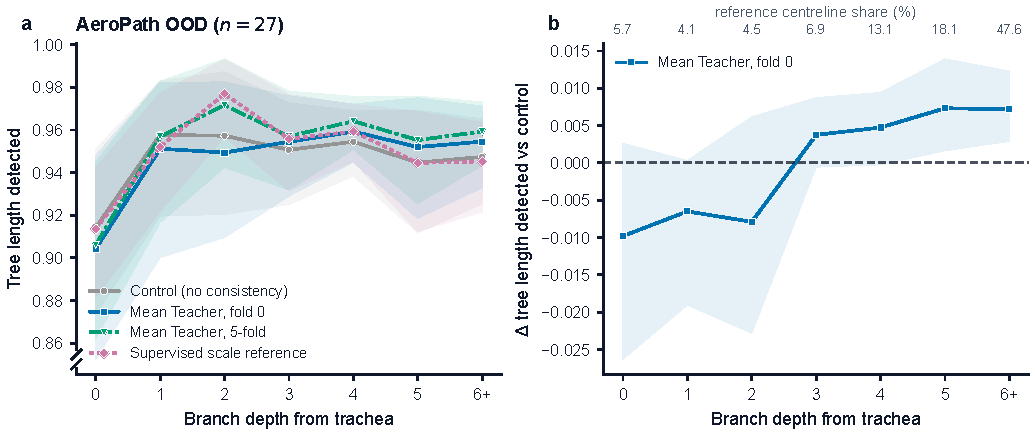
\includegraphics[width=\linewidth]{Figures/pdf/appendix/generation_depth_recovery_aeropath.pdf}
  \caption[AeroPath recovery by branch depth]{Exploratory AeroPath branch-depth recovery.
  (a)~Absolute profiles; (b)~fold-0 Mean Teacher minus control. Depths $\geq6$ are pooled to
  retain all 27 cases. Parser-labelled support excludes 0.25\% of the plain centreline.}
  \label{fig:aeropath-depth}
\end{figure}

\section{Branch depth against airway calibre}
\label{sec:depth-calibre}

The calibre and depth analyses of Sections~\ref{sec:calibre} and~\ref{sec:depth} localise the
same gain along two coordinates, and Figure~\ref{fig:depth-calibre} says how far those
coordinates are the same one. They are related but not interchangeable. The proximal tree is
almost entirely thick: three quarters of the centreline length at depth zero exceeds sixteen
voxels. From depth four onwards the three-to-four-voxel band holds more than half the tree at
every remaining depth, and the narrowest band takes a growing share of the rest, from 8\% at
depth four to a third at the deepest annotated level. Over the reference centreline the two
coordinates rank-correlate at Spearman $\rho=-0.48$; this is a descriptive statistic over
centreline voxels rather than over patients, so no $p$-value is quoted for it. Depth therefore
predicts calibre only loosely, and neither section is a restatement of the other.

\begin{figure}[htbp]
  \centering
  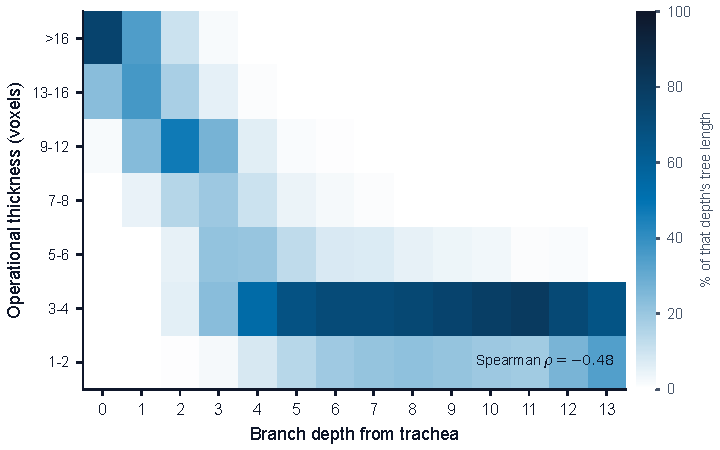
\includegraphics[width=0.86\linewidth]{Figures/pdf/appendix/depth_calibre_heatmap.pdf}
  \caption[Joint distribution of branch depth and airway calibre]{Distribution of reference
  centreline length over operational calibre within each branch depth, on the external
  validation cohort. Each column is normalised to that depth's own tree length, so colour
  reads as the calibre composition of the tree at that depth rather than as its size.}
  \label{fig:depth-calibre}
\end{figure}

\section{Preliminary from-scratch study (superseded)}

% This entire section is material REMOVED from the body during the 2026-08-14 rewire. It is
% retained because the runs happened and the repository contains them, and because a reader
% of the code should be able to reconcile what they find with what the body claims. It is
% NOT part of the dissertation's argument. Keep it descriptive and clearly time-stamped, and
% do not let any body chapter cite a number from here as evidence.

\begin{itemize}
  \item Purpose statement, written defensively: an earlier phase of the project trained a
  from-scratch 3D U-Net under a fixed low-label budget to explore topology-aware objectives
  before a self-configuring pipeline was adopted. It is reported for completeness and to
  document the pivot, not as evidence for any claim in the body.
  \item Configuration: MONAI 3D U-Net, channels $[32,64,128,256,512]$, four stride-2 stages,
  two residual units per level, instance normalisation, PReLU, dropout 0.1; $96^3$ patches,
  foreground-centred sampling probability 0.7, AdamW at $3\times10^{-4}$ with cosine decay and
  mixed precision.
  \item Objective: weighted cross-entropy plus soft Dice, with topology terms withheld for 15
  epochs and ramped over the following 10.
  \item Sealed-test result at validation-fixed thresholds (baseline 0.70, topology variants
  0.50), connected output: baseline hard clDice 0.383, TLD 0.289, topology precision 0.587,
  Dice 0.645, BD 0.229; centreline-loss variant 0.656, 0.592, 0.753, 0.517, 0.451; combined
  centreline plus radius-aware variant 0.709, 0.612, 0.860, 0.560, 0.467.
  \item State the one durable observation and stop there: overlap ranking and tree-completeness
  ranking disagreed sharply in that low-label regime --- the highest-Dice model recovered the
  least reference tree.
  \item State the reason it is superseded, plainly: a supervised nnU-Net trained on the same
  data exceeded these models on every axis including the topology metrics, so absolute airway
  quality in that study was pipeline-bound rather than loss-bound. That result is what
  motivated moving the entire study onto nnU-Net.
  \item Note the post-processing dependence that makes those numbers hard to compare forward:
  at the operating threshold the connected component carried most of the final overlap score
  for the centreline-loss model.
\end{itemize}

\section{Retired ablations (from-scratch pipeline)}

% All negative or inert. Kept as a compact record so the repository is legible and so the
% Discussion can say "these levers were tested" without spending body words on them.

\begin{itemize}
  \item \textbf{Larger patches.} $96^3$ to $128^3$ at otherwise matched settings regressed
  topology (hard clDice 0.683 to 0.334; TLD 0.608 to 0.224) while raising connected Dice
  0.518 to 0.616. The model became conservative rather than sharper. Negative as run, with
  unretuned sampling and epoch count as the stated caveat.
  \item \textbf{Reduced downsampling.} An architecture with a higher-resolution bottleneck
  reproduced the same trade almost exactly: hard clDice 0.516, TLD 0.430, connected Dice
  0.624. Two independent routes to more spatial fidelity both traded tree completeness for
  cleaner proximal masks.
  \item \textbf{Radius-aware objective.} Reduced dependence on connected-component
  post-processing substantially, but at matched tree completeness the final connected masks
  were tied with the centreline-only model, and the geometry-corrected version did not improve
  the balanced model. Retired as a forward lever.
  \item \textbf{Distal sampling and calibre weighting.} Behaved as over-painting rather than
  additional reach; failed their pre-specified decision rules.
  \item \textbf{Gap-bridging reconnection.} Changed tree-length and clDice only at noise scale
  at the tested gap size; the material deleted by connected-component selection was
  predominantly false-positive over-segmentation rather than orphaned true tree.
  \item \textbf{Early semi-supervised arms.} Record the sampler fault --- uniform case
  sampling made all-ignore cases produce batches with no supervised gradient during a long
  warm-up --- and state that the affected arm is excluded from all comparisons as an
  implementation failure rather than a scientific result. Record likewise the loss-ablation
  run truncated at epoch 319 of 1000, whose external score is an early-checkpoint snapshot.
  \item Frame the set honestly in one closing line: these constrain the mechanism by showing
  which levers did not move the completeness/precision frontier, and they informed the
  decision to attack the problem from the data side rather than the loss side.
\end{itemize}

\section{Reproducibility checklist}

\begin{itemize}
  \item Repository layout and exact commands for preprocessing, training, prediction and
  scoring; no machine-specific paths or credentials.
  \item Checksums for final checkpoints, split manifests, prediction bundles and score files;
  note the trainer-source hash pinning used by the launch guards.
  \item Document the known provenance gap --- generated prediction metadata does not record
  trainer, folds or checkpoint filename --- and the convergent evidence used to establish
  checkpoint provenance for affected historical prediction sets.
  \item Unit and integration test summary, including geometry, scoring, ignore-label and
  two-stream provenance tests, plus known deviations from deterministic execution.
  \item Data-access instructions and licence constraints; no redistribution of source scans
  where prohibited.
\end{itemize}

\section{Additional ethical analysis}

\begin{itemize}
  \item Map the main-text discussion onto the six required domains explicitly: scientific
  integrity, collegiality, human subjects, animal welfare, institutional integrity and social
  responsibility --- so the mapping is auditable even where the body text is compressed.
  \item Dataset provenance, licences and source approvals in full.
  \item Extended stakeholder analysis, and the compute/environmental accounting summarised in
  the body.
\end{itemize}

\section{Paired significance tests}

Every significance claim in Chapter~\ref{ch:results} resolves to a row of
Table~\ref{tab:paired-tests}. Because each cohort is scored per case, all comparisons are
paired by case identifier: the statistic is a two-sided paired $t$-test of the per-case
differences against zero, $t=\bar d/(s_d/\sqrt n)$ with $\mathrm{df}=n-1$. Five metrics are
tested per contrast, so a Bonferroni-adjusted $p$-value is given alongside the raw one and
\emph{the adjusted column is what licenses the word significant}. The paired $t$ assumes
approximately normal differences, which is not guaranteed for bounded metrics at $n=20$; a
distribution-free Wilcoxon signed-rank $p$ is therefore reported beside it, and where the two
disagree the Wilcoxon result is the one to quote. Cohen's $d_z=\bar d/s_d$ gives the paired
effect size, and the final column counts cases favouring the arm over its reference.

A limitation applies to every row and is stated once here: these tests quantify consistency
\emph{across patients}, not across training runs. Each arm is a single training run at a
single seed, so a unanimous win count shows that an effect is diffuse rather than carried by
one or two cases; it does not establish that retraining at another seed would reproduce it.

% The complete table environment is generated: \input inside a tabular alignment is a TeX
% error ("Missing \cr inserted"), so the script emits caption, label and all. Re-run
% dissertation/scripts/statistics/paired_significance_tests.py to update it; never hand-edit.
% GENERATED by dissertation/scripts/statistics/paired_significance_tests.py.
% Do not edit: re-run the script so the table and the data stay in agreement.
\begin{table}[htbp]
  \centering
  \scriptsize
  \setlength{\tabcolsep}{3pt}
  \caption[Paired significance tests for every claimed comparison]{Paired
  significance tests for every comparison claimed in this dissertation, on the native
  (RAW) mask. $\bar d$ is the mean per-case difference, arm minus reference. Stars mark
  the Bonferroni-adjusted $p$: ${*}\,p<0.05$, ${**}\,p<0.01$, ${***}\,p<0.001$.
  Generated by \texttt{dissertation/scripts/statistics/paired\_significance\_tests.py}.}
  \label{tab:paired-tests}
  \begin{tabular}{lrcrrrrrrr}
    \toprule
    Metric & $\bar d$ & 95\% CI & $t$ & df & $p$ & $p_{\text{adj}}$ & Wilcoxon & $d_z$ & wins \\
    \midrule
    \multicolumn{10}{l}{\itshape development: probability target vs no-consistency control} \\
    \quad Dice & $-0.0039$ & $[-0.0077,\,-0.0001]$ & $-2.17$ & 19 & $0.0428$ & $0.2139$ & $0.0441$ & $-0.49$ & 7/20 \\
    \quad TLD & $+0.0196$ & $[+0.0147,\,+0.0245]$ & $+8.42$ & 19 & $<\!10^{-4}$ & $<\!10^{-4}$*** & $<\!10^{-4}$ & $+1.88$ & 20/20 \\
    \quad BD & $+0.0362$ & $[+0.0232,\,+0.0491]$ & $+5.84$ & 19 & $<\!10^{-4}$ & $<\!10^{-4}$*** & $<\!10^{-4}$ & $+1.31$ & 19/20 \\
    \quad Prec. & $+0.0057$ & $[-0.0015,\,+0.0129]$ & $+1.66$ & 19 & $0.1129$ & $0.5647$ & $0.1536$ & $+0.37$ & 13/20 \\
    \quad clDice & $-0.0012$ & $[-0.0065,\,+0.0041]$ & $-0.48$ & 19 & $0.6376$ & $1.0000$ & $0.7012$ & $-0.11$ & 9/20 \\
    \addlinespace
    \multicolumn{10}{l}{\itshape development: thresholded target, 5 folds vs no-consistency control} \\
    \quad Dice & $+0.0041$ & $[-0.0053,\,+0.0134]$ & $+0.91$ & 19 & $0.3738$ & $1.0000$ & $0.0897$ & $+0.20$ & 14/20 \\
    \quad TLD & $+0.0190$ & $[+0.0152,\,+0.0228]$ & $+10.47$ & 19 & $<\!10^{-4}$ & $<\!10^{-4}$*** & $<\!10^{-4}$ & $+2.34$ & 20/20 \\
    \quad BD & $+0.0348$ & $[+0.0232,\,+0.0465]$ & $+6.27$ & 19 & $<\!10^{-4}$ & $<\!10^{-4}$*** & $<\!10^{-4}$ & $+1.40$ & 20/20 \\
    \quad Prec. & $+0.0154$ & $[+0.0035,\,+0.0273]$ & $+2.72$ & 19 & $0.0137$ & $0.0683$ & $0.0002$ & $+0.61$ & 17/20 \\
    \quad clDice & $+0.0051$ & $[+0.0013,\,+0.0090]$ & $+2.80$ & 19 & $0.0115$ & $0.0576$ & $0.0136$ & $+0.63$ & 14/20 \\
    \addlinespace
    \multicolumn{10}{l}{\itshape development: thresholded target, 5 folds vs 110-label supervised} \\
    \quad Dice & $+0.0055$ & $[-0.0020,\,+0.0131]$ & $+1.53$ & 19 & $0.1433$ & $0.7166$ & $0.1231$ & $+0.34$ & 13/20 \\
    \quad TLD & $+0.0059$ & $[+0.0009,\,+0.0109]$ & $+2.45$ & 19 & $0.0241$ & $0.1205$ & $0.0242$ & $+0.55$ & 14/20 \\
    \quad BD & $+0.0079$ & $[-0.0023,\,+0.0181]$ & $+1.62$ & 19 & $0.1228$ & $0.6139$ & $0.1089$ & $+0.36$ & 12/20 \\
    \quad Prec. & $+0.0020$ & $[-0.0119,\,+0.0159]$ & $+0.31$ & 19 & $0.7635$ & $1.0000$ & $0.7841$ & $+0.07$ & 8/20 \\
    \quad clDice & $-0.0004$ & $[-0.0048,\,+0.0040]$ & $-0.21$ & 19 & $0.8353$ & $1.0000$ & $0.6742$ & $-0.05$ & 9/20 \\
    \addlinespace
    \multicolumn{10}{l}{\itshape development: probability target, $\beta{=}2$ vs probability target} \\
    \quad Dice & $-0.0743$ & $[-0.1465,\,-0.0020]$ & $-2.15$ & 19 & $0.0446$ & $0.2228$ & $0.0037$ & $-0.48$ & 5/20 \\
    \quad TLD & $+0.0230$ & $[+0.0108,\,+0.0353]$ & $+3.94$ & 19 & $0.0009$ & $0.0044$** & $<\!10^{-4}$ & $+0.88$ & 18/20 \\
    \quad BD & $+0.0475$ & $[+0.0187,\,+0.0763]$ & $+3.45$ & 19 & $0.0027$ & $0.0133$* & $0.0005$ & $+0.77$ & 16/20 \\
    \quad Prec. & $-0.1357$ & $[-0.2266,\,-0.0448]$ & $-3.12$ & 19 & $0.0056$ & $0.0280$* & $<\!10^{-4}$ & $-0.70$ & 0/20 \\
    \quad clDice & $-0.1823$ & $[-0.2888,\,-0.0757]$ & $-3.58$ & 19 & $0.0020$ & $0.0100$** & $<\!10^{-4}$ & $-0.80$ & 0/20 \\
    \addlinespace
    \multicolumn{10}{l}{\itshape sealed test: probability target vs no-consistency control} \\
    \quad Dice & $-0.0008$ & $[-0.0059,\,+0.0042]$ & $-0.35$ & 19 & $0.7301$ & $1.0000$ & $0.8408$ & $-0.08$ & 10/20 \\
    \quad TLD & $+0.0181$ & $[+0.0126,\,+0.0236]$ & $+6.90$ & 19 & $<\!10^{-4}$ & $<\!10^{-4}$*** & $<\!10^{-4}$ & $+1.54$ & 19/20 \\
    \quad BD & $+0.0379$ & $[+0.0263,\,+0.0495]$ & $+6.85$ & 19 & $<\!10^{-4}$ & $<\!10^{-4}$*** & $<\!10^{-4}$ & $+1.53$ & 19/20 \\
    \quad Prec. & $+0.0104$ & $[+0.0021,\,+0.0187]$ & $+2.64$ & 19 & $0.0163$ & $0.0813$ & $0.0083$ & $+0.59$ & 14/20 \\
    \quad clDice & $-0.0016$ & $[-0.0065,\,+0.0034]$ & $-0.67$ & 19 & $0.5087$ & $1.0000$ & $0.5459$ & $-0.15$ & 8/20 \\
    \addlinespace
    \multicolumn{10}{l}{\itshape sealed test: thresholded target, 5 folds vs no-consistency control} \\
    \quad Dice & $+0.0116$ & $[+0.0051,\,+0.0181]$ & $+3.71$ & 19 & $0.0015$ & $0.0074$** & $<\!10^{-4}$ & $+0.83$ & 16/20 \\
    \quad TLD & $+0.0143$ & $[+0.0097,\,+0.0190]$ & $+6.43$ & 19 & $<\!10^{-4}$ & $<\!10^{-4}$*** & $<\!10^{-4}$ & $+1.44$ & 20/20 \\
    \quad BD & $+0.0300$ & $[+0.0192,\,+0.0407]$ & $+5.85$ & 19 & $<\!10^{-4}$ & $<\!10^{-4}$*** & $0.0002$ & $+1.31$ & 18/20 \\
    \quad Prec. & $+0.0233$ & $[+0.0108,\,+0.0358]$ & $+3.90$ & 19 & $0.0010$ & $0.0048$** & $<\!10^{-4}$ & $+0.87$ & 19/20 \\
    \quad clDice & $+0.0017$ & $[-0.0043,\,+0.0077]$ & $+0.59$ & 19 & $0.5619$ & $1.0000$ & $0.3488$ & $+0.13$ & 13/20 \\
    \addlinespace
    \multicolumn{10}{l}{\itshape sealed test: thresholded target, 5 folds vs 110-label supervised} \\
    \quad Dice & $+0.0067$ & $[-0.0058,\,+0.0193]$ & $+1.12$ & 19 & $0.2749$ & $1.0000$ & $0.4980$ & $+0.25$ & 11/20 \\
    \quad TLD & $+0.0037$ & $[-0.0020,\,+0.0095]$ & $+1.36$ & 19 & $0.1893$ & $0.9466$ & $0.0826$ & $+0.30$ & 14/20 \\
    \quad BD & $+0.0140$ & $[+0.0022,\,+0.0259]$ & $+2.48$ & 19 & $0.0227$ & $0.1133$ & $0.0400$ & $+0.55$ & 15/20 \\
    \quad Prec. & $+0.0145$ & $[-0.0089,\,+0.0379]$ & $+1.29$ & 19 & $0.2110$ & $1.0000$ & $0.7562$ & $+0.29$ & 11/20 \\
    \quad clDice & $-0.0037$ & $[-0.0091,\,+0.0017]$ & $-1.43$ & 19 & $0.1692$ & $0.8459$ & $0.2774$ & $-0.32$ & 8/20 \\
    \addlinespace
    \multicolumn{10}{l}{\itshape sealed test: probability target, $\beta{=}2$ vs no-consistency control} \\
    \quad Dice & $-0.0575$ & $[-0.0883,\,-0.0267]$ & $-3.91$ & 19 & $0.0009$ & $0.0047$** & $<\!10^{-4}$ & $-0.87$ & 0/20 \\
    \quad TLD & $+0.0348$ & $[+0.0265,\,+0.0431]$ & $+8.80$ & 19 & $<\!10^{-4}$ & $<\!10^{-4}$*** & $<\!10^{-4}$ & $+1.97$ & 20/20 \\
    \quad BD & $+0.0654$ & $[+0.0485,\,+0.0822]$ & $+8.14$ & 19 & $<\!10^{-4}$ & $<\!10^{-4}$*** & $<\!10^{-4}$ & $+1.82$ & 20/20 \\
    \quad Prec. & $-0.1097$ & $[-0.1547,\,-0.0646]$ & $-5.10$ & 19 & $<\!10^{-4}$ & $0.0003$*** & $<\!10^{-4}$ & $-1.14$ & 0/20 \\
    \quad clDice & $-0.1503$ & $[-0.2254,\,-0.0752]$ & $-4.19$ & 19 & $0.0005$ & $0.0025$** & $<\!10^{-4}$ & $-0.94$ & 0/20 \\
    \addlinespace
    \multicolumn{10}{l}{\itshape AeroPath: probability target vs no-consistency control} \\
    \quad Dice & $+0.0002$ & $[-0.0068,\,+0.0073]$ & $+0.06$ & 26 & $0.9511$ & $1.0000$ & $0.6964$ & $+0.01$ & 16/27 \\
    \quad TLD & $+0.0057$ & $[+0.0012,\,+0.0102]$ & $+2.59$ & 26 & $0.0155$ & $0.0774$ & $0.0082$ & $+0.50$ & 17/27 \\
    \quad BD & $+0.0132$ & $[+0.0041,\,+0.0222]$ & $+3.00$ & 26 & $0.0059$ & $0.0297$* & $0.0046$ & $+0.58$ & 15/27 \\
    \quad Prec. & $+0.0143$ & $[+0.0035,\,+0.0251]$ & $+2.71$ & 26 & $0.0116$ & $0.0581$ & $0.0017$ & $+0.52$ & 20/27 \\
    \quad clDice & $-0.0232$ & $[-0.0358,\,-0.0107]$ & $-3.81$ & 26 & $0.0008$ & $0.0038$** & $0.0007$ & $-0.73$ & 4/27 \\
    \addlinespace
    \multicolumn{10}{l}{\itshape AeroPath: thresholded target, 5 folds vs 110-label supervised} \\
    \quad Dice & $-0.0043$ & $[-0.0132,\,+0.0046]$ & $-0.99$ & 26 & $0.3293$ & $1.0000$ & $0.3242$ & $-0.19$ & 9/27 \\
    \quad TLD & $+0.0053$ & $[+0.0015,\,+0.0091]$ & $+2.85$ & 26 & $0.0085$ & $0.0423$* & $0.0013$ & $+0.55$ & 23/27 \\
    \quad BD & $+0.0034$ & $[-0.0017,\,+0.0084]$ & $+1.36$ & 26 & $0.1840$ & $0.9198$ & $0.1788$ & $+0.26$ & 11/27 \\
    \quad Prec. & $-0.0177$ & $[-0.0217,\,-0.0137]$ & $-9.00$ & 26 & $<\!10^{-4}$ & $<\!10^{-4}$*** & $<\!10^{-4}$ & $-1.73$ & 1/27 \\
    \quad clDice & $-0.0279$ & $[-0.0356,\,-0.0202]$ & $-7.47$ & 26 & $<\!10^{-4}$ & $<\!10^{-4}$*** & $<\!10^{-4}$ & $-1.44$ & 2/27 \\
    \addlinespace
    \bottomrule
  \end{tabular}
\end{table}


% ---------------------------------------------------------------------------
% SUPPLEMENTARY FIGURES (added 2026-08-21). Every figure here is generated by a
% script under dissertation/scripts/ and carries a provenance record under
% Figures/provenance/. Re-run the named script to update one; never edit a PDF.
%
% They are parked at the END OF THE APPENDIX on purpose. The body is capped at
% twenty figures and tables, the appendix is excluded from that cap, and several
% of these depend on arms that are still training. Promoting one into the body is
% a matter of moving its figure environment into the relevant Results section and
% re-running its script with --pdf-output-dir Figures/pdf/results.
%
% FloatBarrier after each group keeps them in the order they are written rather
% than letting LaTeX reorder a queue of fifteen floats.
% ---------------------------------------------------------------------------
\section{Supplementary figures}
\label{sec:supplementary-figures}

The figures collected here support claims the body states in prose or in a table of means.
They are grouped by what they are evidence for rather than by the order they were produced:
the consistency objective, the position of the arms against supervised scale, the
patient-level distribution of the treatment effect, what the difference looks like on an
airway, and the two behaviours --- component filtering and training-run variation --- that
bound how far the result can be read.

Each is generated from the per-case score files and prediction masks already on disk. The
generating script is named in every caption, and each writes a provenance record under
\texttt{Figures/provenance/} listing the exact prediction directories it read.

\subsection{Consistency objective and supervision scale}
\label{sec:supp-objective}

Section~\ref{sec:ablation-mse} asks whether the gain requires a topology-aware consistency
objective or would follow from unlabelled consistency of any form.
Figure~\ref{fig:supp-objective-val} answers it in the paired form the rest of the chapter
uses: both objectives are shown as differences from the \emph{same} no-consistency
comparator, rather than against each other, so the matched-comparator logic is preserved.

Both objectives are drawn at the same consistency weight, $w_{\max}=0.10$, so the two rows
differ in the consistency distance alone; the weight each arm carries is printed on its own
tick label rather than left to a footnote. The two arms are nonetheless independently
realised training runs, as is the comparator they are both differenced against, so the
figure shows consistency across patients and not across training seeds.

\begin{figure}[htbp]
  \centering
  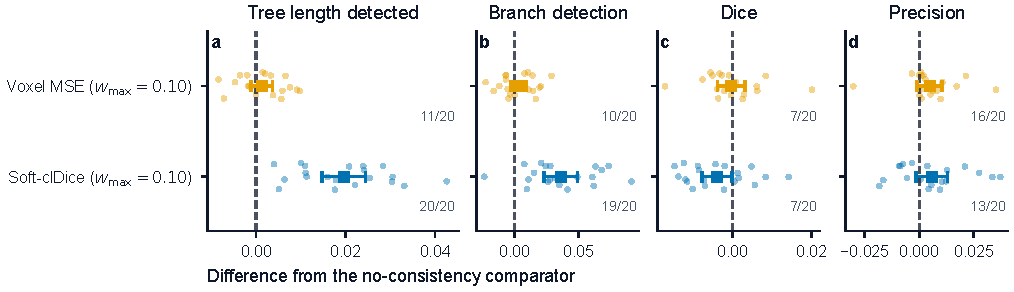
\includegraphics[width=\linewidth]{Figures/pdf/appendix/objective_comparison_val.pdf}
  \caption[Consistency objective, paired against the no-consistency comparator]{Centreline
  against voxelwise consistency on the external validation cohort, each as a paired per-case
  difference from the same no-consistency comparator. Points are patients, squares are means
  with 95\% intervals, and the fraction at the right of each row counts patients favouring
  that arm. Both arms run at $w_{\max}=0.10$: the weight each carries is printed on its own
  label. Both are single training runs, independently realised from the comparator, so this
  is consistency across patients rather than across seeds. Generated by
  \texttt{dissertation/scripts/plot\_arm\_comparison.py}.}
  \label{fig:supp-objective-val}
\end{figure}

\begin{figure}[htbp]
  \centering
  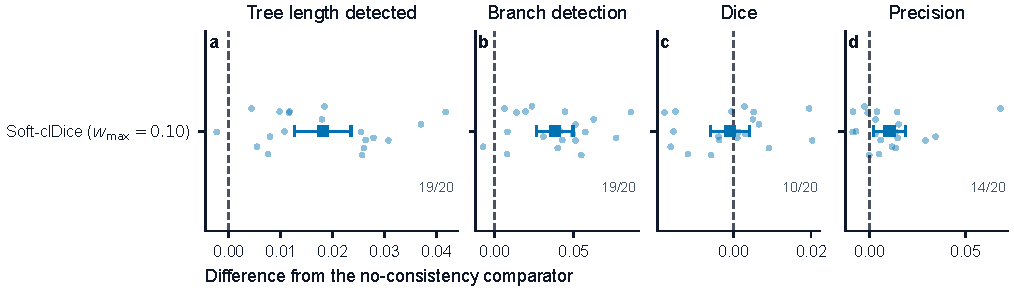
\includegraphics[width=\linewidth]{Figures/pdf/appendix/objective_comparison_test.pdf}
  \caption[Consistency objective on the held-out cohort]{The same contrast on the sealed
  ATM'22 test cohort. Only the centreline objective appears: the voxel-MSE arm has not been
  scored outside the development cohort, and no row is drawn for an arm that has no numbers.}
  \label{fig:supp-objective-test}
\end{figure}

\FloatBarrier

Figure~\ref{fig:supp-scale-val} places the semi-supervised arms against models trained from
larger labelled pools. The shaded rows are a \emph{scale reference} and nothing more. They
differ from the treated arms in labelled-case count, in internal fold membership and in
training protocol at once, so the distance to them is not a label-efficiency measurement,
does not isolate the effect of label count, and is not evidence of equivalence at any point.

\begin{figure}[htbp]
  \centering
  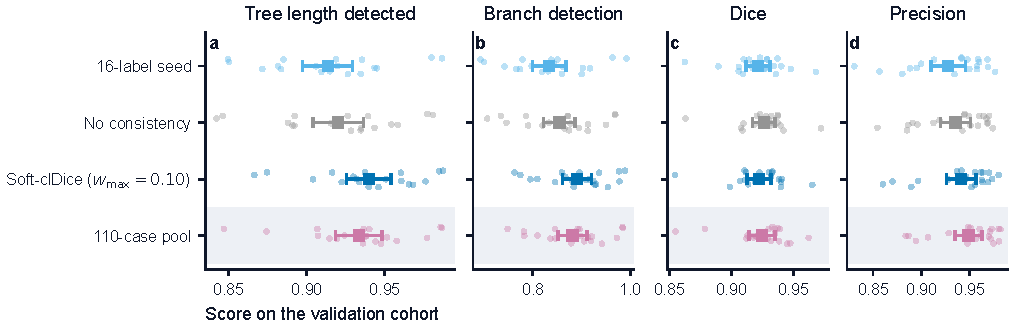
\includegraphics[width=\linewidth]{Figures/pdf/appendix/supervision_scale_val.pdf}
  \caption[Arms against the supervised scale reference, validation cohort]{Per-case scores
  with cohort means and 95\% intervals, external validation cohort. The shaded row is a
  supervised scale reference: it is confounded with fold membership and training protocol,
  so the gap to it is not a matched label-efficiency curve and no equivalence is claimed.
  Generated by \texttt{dissertation/scripts/plot\_arm\_comparison.py}.}
  \label{fig:supp-scale-val}
\end{figure}

\begin{figure}[htbp]
  \centering
  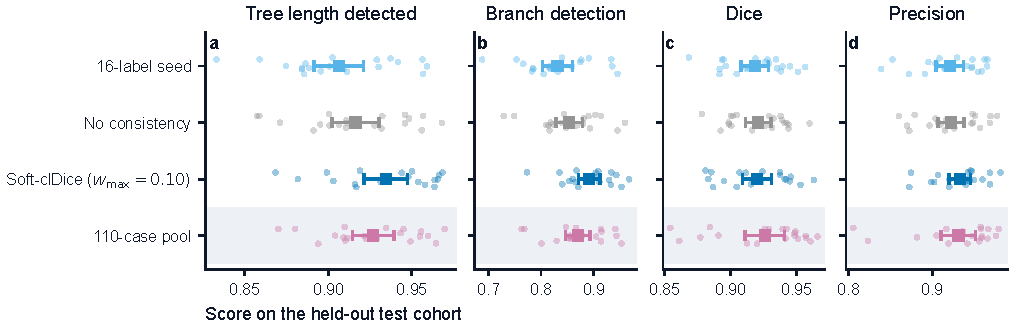
\includegraphics[width=\linewidth]{Figures/pdf/appendix/supervision_scale_test.pdf}
  \caption[Arms against the supervised scale reference, held-out cohort]{The same panel on
  the sealed ATM'22 test cohort. The same caveat applies unchanged.}
  \label{fig:supp-scale-test}
\end{figure}

\FloatBarrier

% Figure~\ref{fig:supp-objective-scale} is the two preceding pairs STACKED. It exists so that
% one slot can carry both arguments if the body ever needs it. Delete it, or delete the four
% figures above it -- do not submit both.
Figure~\ref{fig:supp-objective-scale} stacks the two arguments into a single figure, for the
case where one slot has to carry both. It contains no data the four preceding figures do not.

\begin{figure}[htbp]
  \centering
  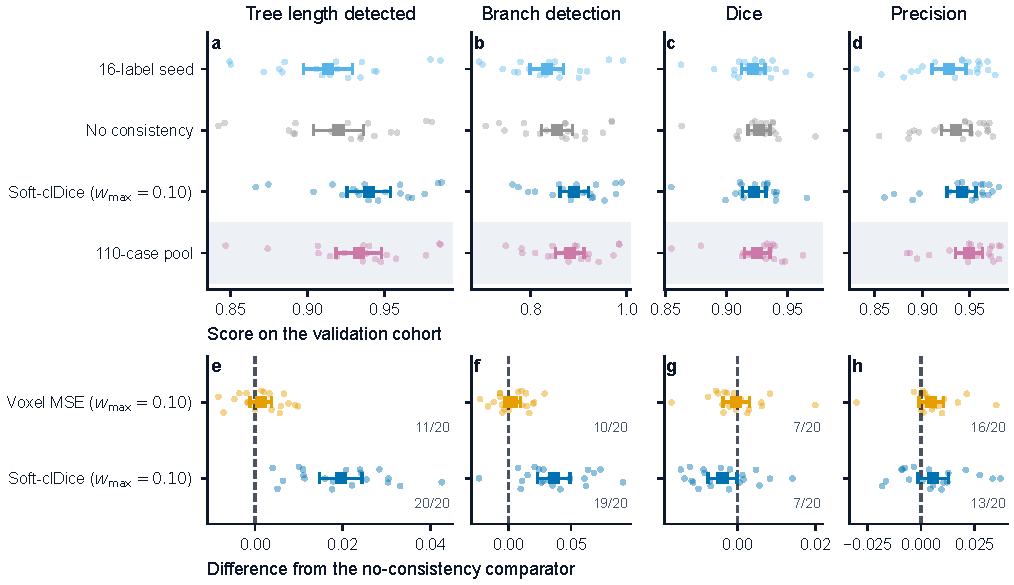
\includegraphics[width=\linewidth]{Figures/pdf/appendix/objective_and_scale_val.pdf}
  \caption[Objective comparison and supervision scale together]{Top row: where each arm sits
  on the external validation cohort, with the supervised scale reference shaded. Bottom row:
  the two consistency objectives as paired differences from the same no-consistency
  comparator. A combined form of Figures~\ref{fig:supp-objective-val}
  and~\ref{fig:supp-scale-val}.}
  \label{fig:supp-objective-scale}
\end{figure}

\FloatBarrier

\subsection{Patient-level treatment effect across cohorts}
\label{sec:supp-paired}

Sections~\ref{sec:primary-matched-pair} and~\ref{sec:external} support two claims with win
counts and cohort means: that the gain is diffuse rather than carried by a few patients, and
that it survives a change of cohort. Both are claims about a \emph{distribution} of paired
differences, which neither a mean nor a win count can show.

Figure~\ref{fig:supp-paired-summary} puts the three cohorts on one axis per metric, so the
effect sizes are compared directly rather than across three tables. AeroPath is drawn beside
the two ATM'22 cohorts but never pooled with them: it is a different scanner and a different
annotation protocol, and the visibly smaller topology difference there is the honest reading
of the out-of-distribution result.

Figure~\ref{fig:supp-paired-cases} then names every patient. All three panels share one
difference axis; the row pitch differs because the cohorts hold different numbers of
patients.

\begin{figure}[htbp]
  \centering
  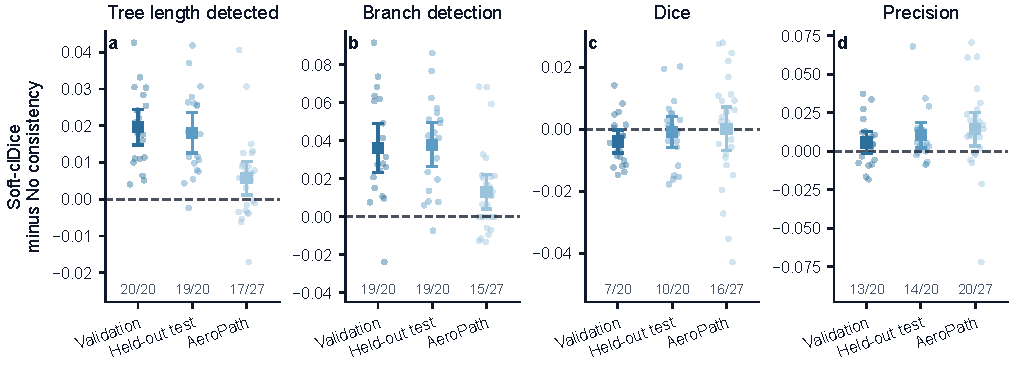
\includegraphics[width=\linewidth]{Figures/pdf/appendix/paired_effect_summary_soft_f0.pdf}
  \caption[Treatment effect by cohort]{Fold-0 Mean Teacher minus its no-consistency
  comparator, on the external validation, sealed test and AeroPath cohorts. Points are
  patients, squares are means with 95\% intervals, and the fraction on the floor of each
  panel counts patients favouring the treatment. Both arms are single training runs, so this
  is consistency across patients, not across seeds. Generated by
  \texttt{dissertation/scripts/plot\_paired\_effects.py}.}
  \label{fig:supp-paired-summary}
\end{figure}

\begin{figure}[htbp]
  \centering
  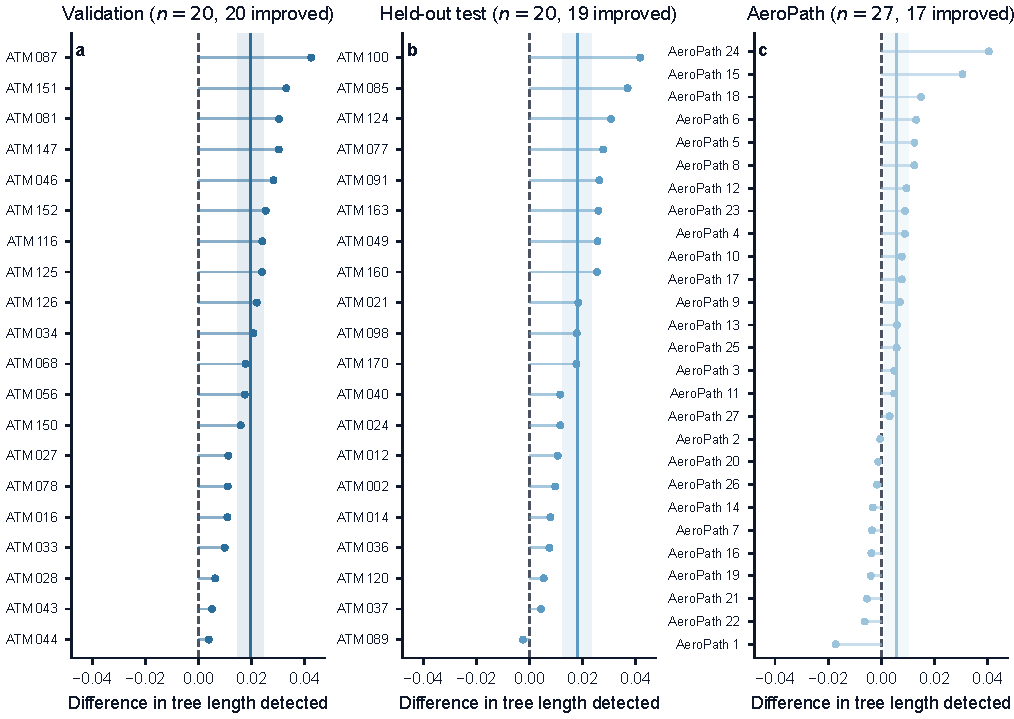
\includegraphics[width=\linewidth]{Figures/pdf/appendix/paired_effect_cases_soft_f0_td_raw.pdf}
  \caption[Per-patient difference in tree length detected]{Every patient's paired difference
  in tree length detected, ordered within each cohort. The vertical line is the cohort mean
  and the band its 95\% interval; all three panels share one difference axis. The
  distribution, not one or two patients, carries the validation and held-out results; on
  AeroPath the effect is smaller and ten of 27 patients fall on the other side of zero.}
  \label{fig:supp-paired-cases}
\end{figure}

\FloatBarrier

\subsection{What the difference looks like on an airway}
\label{sec:supp-qualitative}

A difference of $+0.02$ in tree length detected is not something a reader can picture. The
median-patient render is therefore shown in Figure~\ref{fig:supp-qualitative} in the Discussion,
with supporting cases retained here. Every panel uses the Introduction's isosurface and shading
and one shared screen frame, so the trees overlay pixel for pixel and only the colouring differs.

\textbf{Patients are chosen by a stated rule, never by eye.} Cases are ranked by their own
paired difference in tree length detected, and the rule names a position in that ranking:
Figure~\ref{fig:supp-qualitative} draws the median patient of the validation cohort and
Figure~\ref{fig:supp-error-classes} the largest gain. The complete ranking, including every
patient not drawn, is written to \texttt{Figures/provenance/case\_gallery\_val.json}.

The change panel of Figure~\ref{fig:supp-qualitative} classifies the reference
\emph{centreline}, not reference voxels, because tree length detected is centreline recall:
recovered minus lost, over skeleton length, reproduces the reported paired difference
exactly. A voxel-basis panel would instead be dominated by single-voxel disagreement along
the walls of large airways, which is not what the metric counts.

\begin{figure}[htbp]
  \centering
  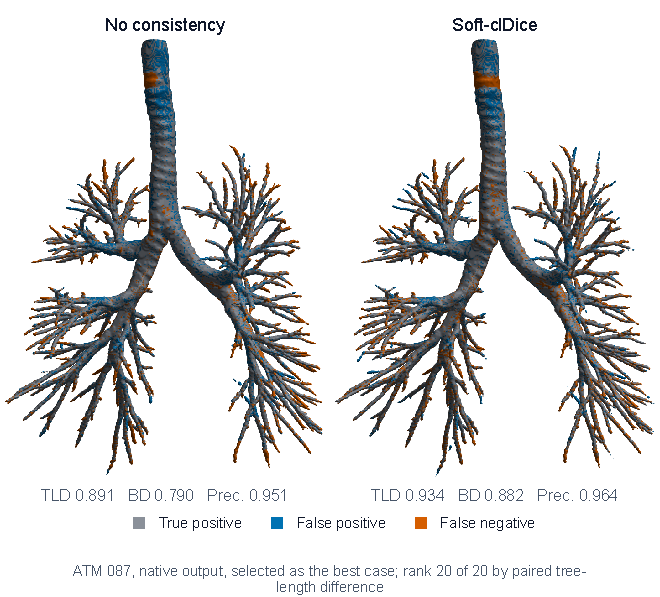
\includegraphics[width=0.65\linewidth]{Figures/pdf/appendix/error_classes_val_control_soft_f0_087.pdf}
  \caption[Voxel error classes for both arms on one patient]{ATM~087, the largest paired
  tree-length gain in the validation cohort, with both arms coloured by voxel error class in
  one shared frame. The distal tips carry the difference: whole terminal branches that are
  false negative under the comparator are produced by the treated arm. The pervasive
  fine-grained false negative along the walls of large airways is wall-thickness
  disagreement, which tree length detected does not count.}
  \label{fig:supp-error-classes}
\end{figure}

\FloatBarrier

\begin{figure}[htbp]
  \centering
  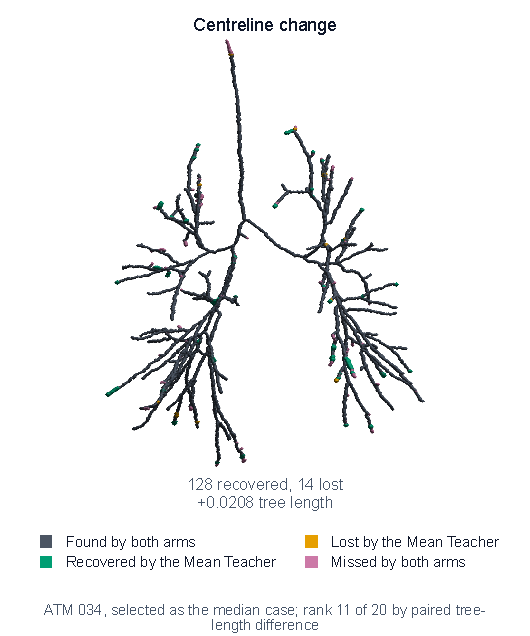
\includegraphics[width=0.52\linewidth]{Figures/pdf/appendix/distal_recovery_val_034.pdf}
  \caption[Distal recovery on the median validation patient]{The change panel of
  Figure~\ref{fig:supp-qualitative} at full width. Recovery is concentrated at the terminal
  branches; the pale class is reference centreline that neither arm produced.}
  \label{fig:supp-recovery-val}
\end{figure}

\begin{figure}[htbp]
  \centering
  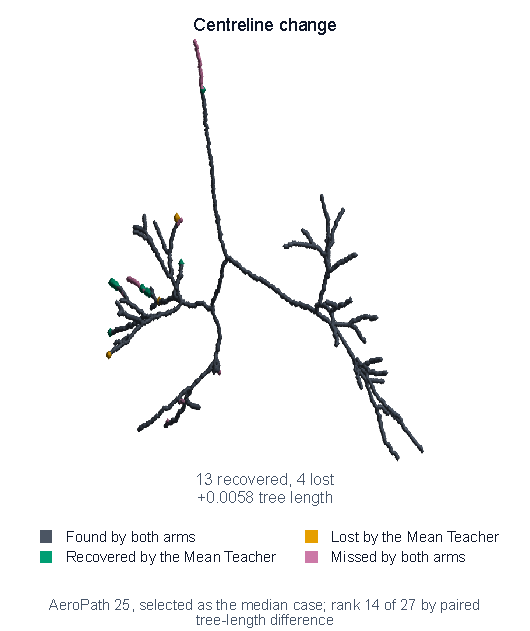
\includegraphics[width=0.52\linewidth]{Figures/pdf/appendix/distal_recovery_ood_925.pdf}
  \caption[Distal recovery out of distribution]{The same panel for AeroPath~25, the median
  patient of that cohort. The annotated tree is shallower than ATM'22's and the change is
  correspondingly smaller: 13 centreline voxels recovered against four lost, a $+0.0058$
  tree-length difference.}
  \label{fig:supp-recovery-ood}
\end{figure}

\FloatBarrier

\subsection{Connected-component filtering and case~044}
\label{sec:supp-postprocessing}

Every metric in this document is reported twice, native and after a trachea-seeded
connected-component filter, and Section~\ref{sec:primary-matched-pair} states in prose that
the filter can delete a detached but genuine subtree. Figure~\ref{fig:supp-postprocessing}
is that statement drawn. The filter is applied by the same function the scorer calls, at the
same connectivity and with the prediction's own affine, so the picture is of the operation
the LCC columns report rather than of a re-implementation.

The two patients are chosen by what the filter did to them: the largest precision gain and
the largest tree-length loss over the cohort. The second rule selects case~044 without being
told to, which is the independent check on the account given in the Discussion.

\begin{figure}[htbp]
  \centering
  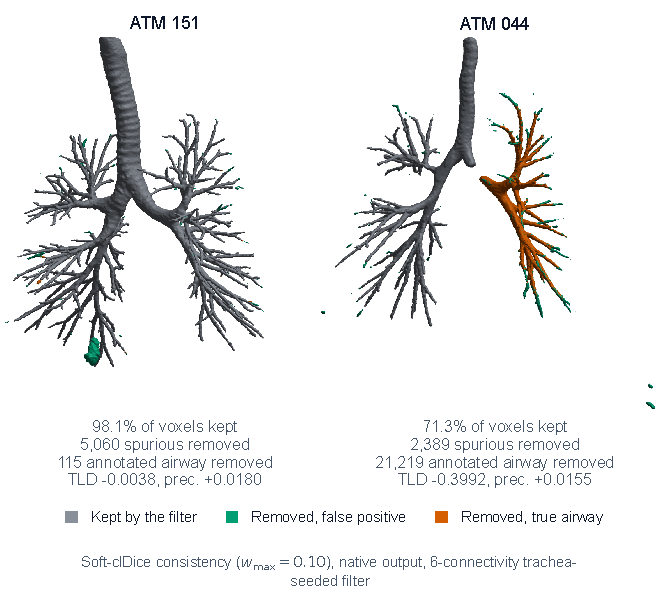
\includegraphics[width=0.65\linewidth]{Figures/pdf/appendix/postprocessing_cases_val_soft_f0.pdf}
  \caption[When component filtering helps and when it deletes airway]{The trachea-seeded
  component filter on two validation patients, each voxel coloured by what the filter did and
  whether it was right to. Left, ATM~151, the largest precision gain in the cohort: the
  filter removes a detached false-positive mass, and 115 annotated airway voxels with it.
  Right, ATM~044: a proximal discontinuity detaches an entire right-lung subtree, and the
  filter deletes 21{,}219 annotated airway voxels, 28.7\% of the prediction, taking tree
  length detected down by $0.3992$. Generated by
  \texttt{dissertation/scripts/render\_postprocessing\_cases.py}.}
  \label{fig:supp-postprocessing}
\end{figure}

\FloatBarrier

\subsection{Training diagnostics}
\label{sec:supp-diagnostics}

Figure~\ref{fig:supp-diagnostics} is descriptive and is labelled as such. The panel that
would matter --- the spread between replicates of one arm, against which the reported
treatment difference has to be read --- requires more than one training run per arm, and the
paired replicate protocol that produces them is still running. The generating script refuses
to draw that panel from a single run and has to be forced past the guard, because a single
trajectory presented as a distribution is precisely the overclaim the protocol exists to
prevent. What is shown instead is one run's optimisation behaviour: the consistency weight
schedule against the gradient it actually produced, and the cosine between the consistency
and supervised gradients.

\begin{figure}[htbp]
  \centering
  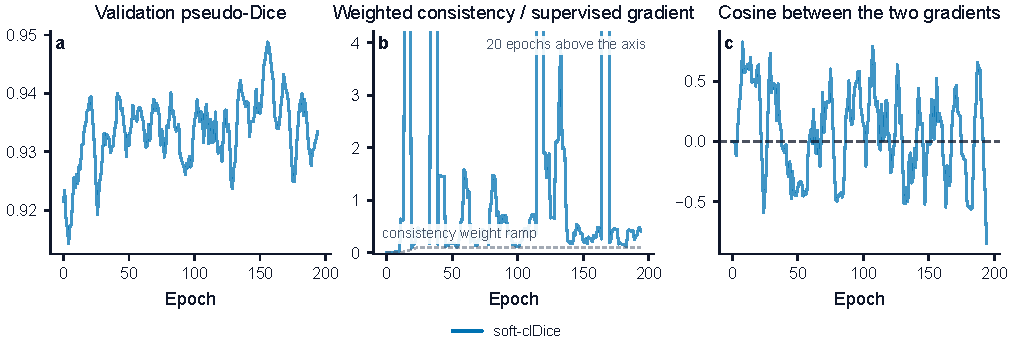
\includegraphics[width=\linewidth]{Figures/pdf/appendix/training_diagnostics_single_run.pdf}
  \caption[Optimisation behaviour of a single Mean Teacher run]{Diagnostics from one
  soft-clDice training run, smoothed with a centred five-epoch mean.
  (a)~nnU-Net's running validation pseudo-Dice.
  (b)~The weighted consistency gradient as a fraction of the supervised one, with the weight
  schedule beneath it; the axis is cut at an interquartile fence and reports how many epochs
  fall above it, all of them steps where the supervised gradient nearly vanished.
  (c)~The cosine between the two gradients, which spends much of training below zero.
  This is a single run and therefore descriptive: it says nothing about run-to-run variation.
  Generated by \texttt{dissertation/scripts/plot\_training\_diagnostics.py}.}
  \label{fig:supp-diagnostics}
\end{figure}

\FloatBarrier
